\documentclass[]{article}
\usepackage{graphicx}
\usepackage{indentfirst}

\usepackage{clrscode3e}
\setlength{\parindent}{0pt}

%clrs code is good!

\title{HW04 for ECE 9343}
\author{Tongda XU, N18100977}

\begin{document}

\maketitle

\section{Question 1: CLRS Exercise 22.1-3}

\begin{codebox}
	\Procname{$\proc{Transpose($Adjlist$)}$}
	\li new $AdjlistPrime$
	\li \For each $node$ in Adjlist
	\li		\Do \For each $subnode$ in $Adjlist(node)$
	\li 		\Do $AdjlistPrime(subnode).insert(node)$
	\li $Adjlist \gets AdjlistPrime$
	\End
\end{codebox}

For adjacent list: just traverse every node and rebuild one\\
$\Theta (E+V)$ for time and space complexity, hard to do it inplace\\

\begin{codebox}
	\Procname{$\proc{Transpose($Adjmatrix$)}$}
	\li \For each $pair(i,j)$ in upper left Adjmatrix
	\li		\Do \proc{Swap($Adjmatrix[i,j], Adjmatrix[j,i]$)}
	\End
\end{codebox}

For adjacent matrix: just transpose the matrix\\
$\Theta (V^2)$ for time and $\Theta(1)$ for space

\section{Question 2: CLRS Exercise 22.1-5}

For adjacent list, it is hard. We should regard it as a \proc{Breadth-first-search($G$)} end at $d = 2$:

\begin{codebox}
	
	\Procname{$\proc{square($G$)}$}
	\li \For each $u$ in $G.vertices$
	\li 	\Do $G.reset()$
	\li     $list = \emptyset$
	\li 	$u.adjlist^{'} = \proc{BFS-Aid($G, u, list, 0$)}$
	\End
	\End
\end{codebox}

\begin{codebox}
	
	\Procname{$\proc{BFS-Aid($G, u, list, dist$)}$}
	\li \For each $v$ in $u.adjlist$
	\li 	\Do \If $v.color = white$ and $dist \le 2$ 
	\li			\Then $list.insert(u)$
	\li 		\proc{BFS-Aid($G, v, list, dist+1$)}
	\End=
	\End
	\li \Return $list$
\end{codebox}

This could cost $\Theta(V^2 + VE)$ time and $\Theta(V+E)$ space (if optimized).\\

For adjacent matrix, the square process would be simple. for each index m of matrix row, if matrix[m][n] exist, calculate bool union of matrix[m] and matrix[n]:

\begin{codebox}
	
	\Procname{$\proc{square($G$)}$}
	\li \For each $m$ in $G.adjMatrix$
	\li \Do \For each $n$ $G.adjMatrix[m]$
	\li 	\Do \If $G.adjMatrix[m][n] == 1$
	\li         \Then $G^{'}.adjMatrix[m]$ = \proc{And($G.adjMatrix[m],G.adjMatrix[n]$)}
	\End
	\End
	\End
	\li \Return $G^{'}$
\end{codebox}

The \proc{square($G$)} cost $\Theta(V^3)$ time and $\Theta(V)$ space (if optimize)

\section{Question 3: CLRS Exercise 22.2-6}

Consider the following condition in Figure ~\ref{fig:22.2-6}: \\
$E_{\pi} = <s, u1>, <u1, v1>, <s, u2>, <u2, v2>$\\
In BFS Tree, $\delta (s, v1), \delta (s, v2) $ is either $<s, u1, v1>, <s, u1, v2>$ or $<s, u2, v1>, <s, u2, v2>$

\begin{figure}
	\centering
	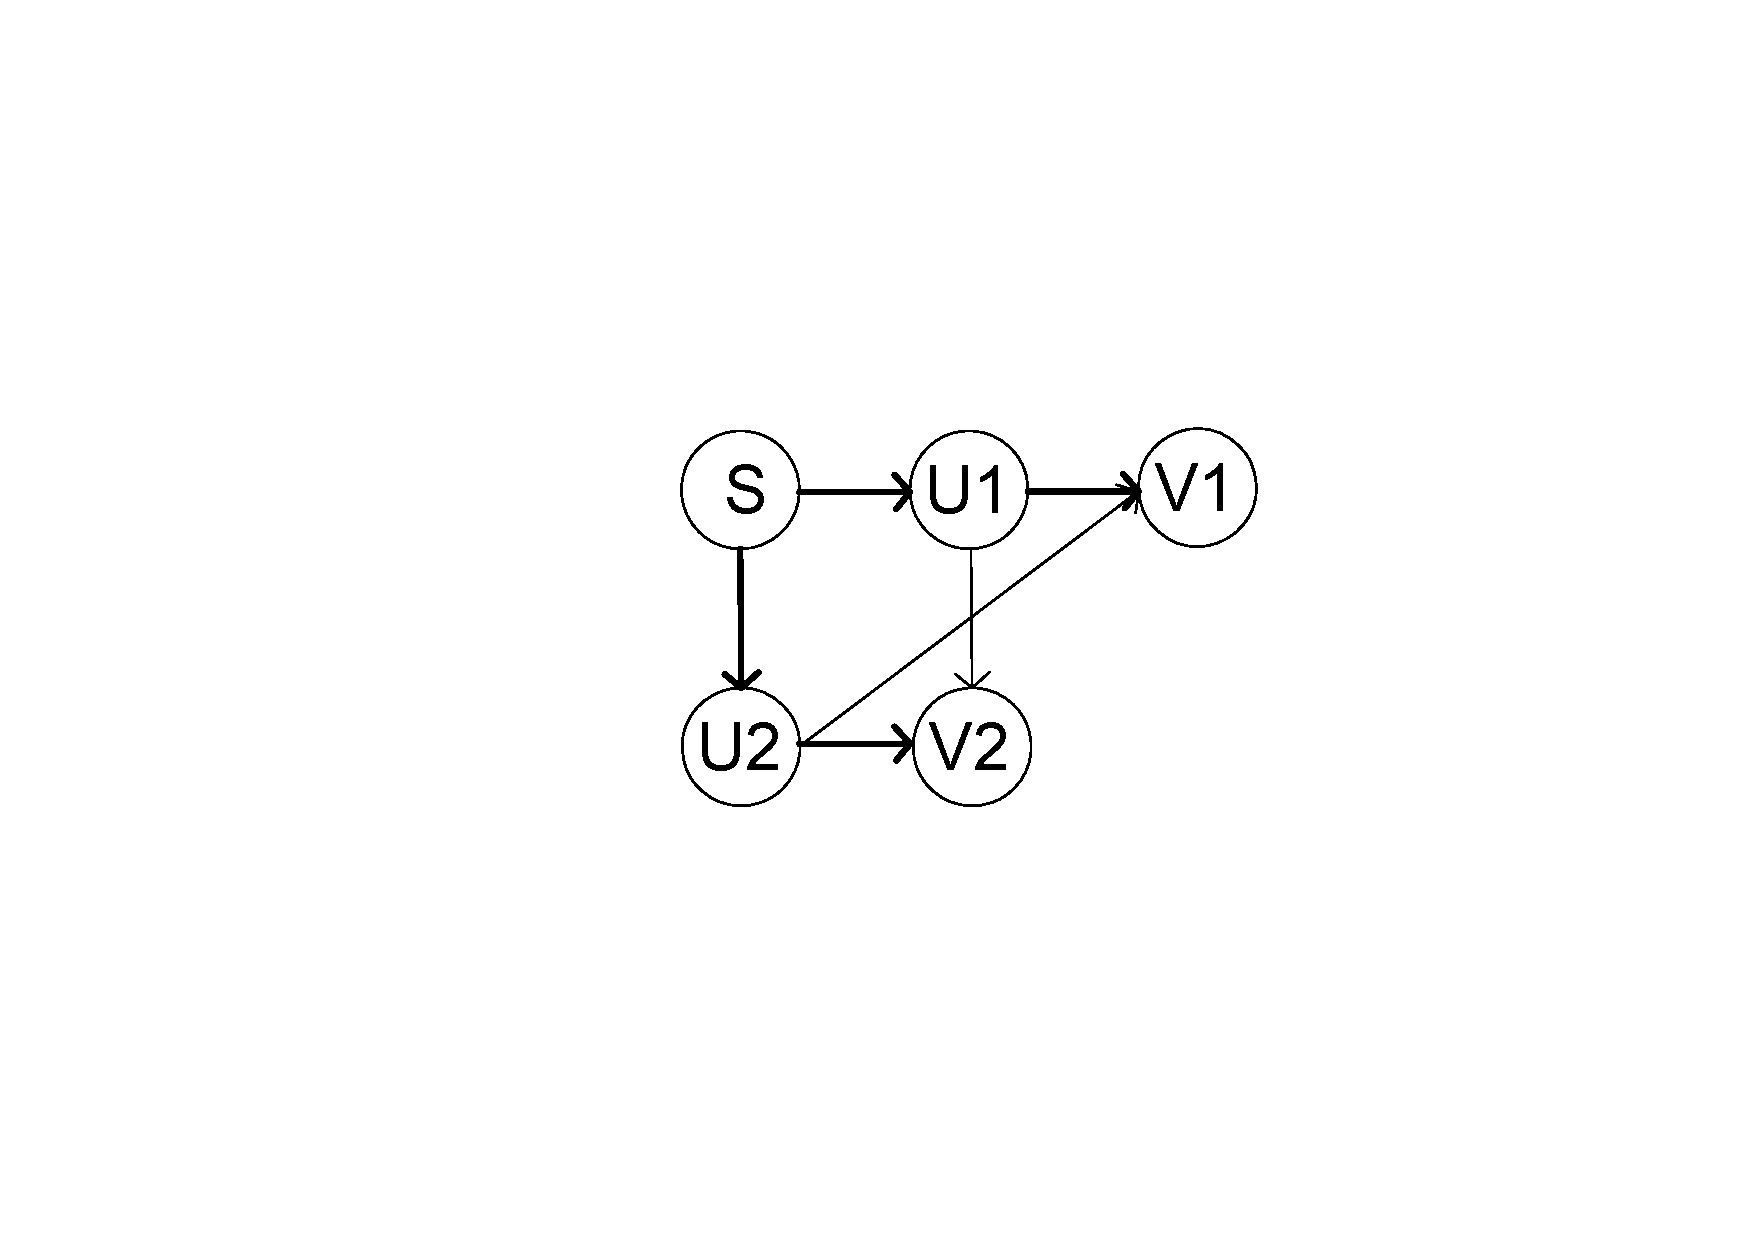
\includegraphics[width=\linewidth]{2226}
	\caption{22.2-6}
	\label{fig:22.2-6}
\end{figure}

\section{Question 4: Traverse Edge of undirected graph}
According to $Theorem 22.10$, all edges are either tree edge or back edge. Modify the \proc{DFS-Visit($G,u$)}, add a \proc{print-path($G,u$)} would do it. Assume a $root = u$ is selected:

\begin{codebox}
	
	\Procname{$\proc{DFS-Visit($G,u$)}$}
	\li $u.color = grey$
	\li $dict[(Vertex,Vertex), edgeType] = \emptyset$
	\li	\For each $v$ in $u.adjList$
	\li \Do \If $v.color == white$
	\li 	\Then $dict(u,v) = treeEdge$
	\li 		  \proc{DFS-Visit($G,v$)}
	\li 	\Else $dict(u,v) = backEgde$
	\End
	\End
	\li \proc{print-path($G,u$)}
	
\end{codebox}

\begin{codebox}
	
	\Procname{$\proc{print-path($G,u$)}$}
	\li \proc{print ($"u"$)}
	\li	\For each $v$ in $u.adjList$
	\li \Do \If $(u,v) == treeedge$
	\li 	\Then \proc{print ($"\rightarrow"$)}
	\li     \proc{print-path($G,v$)}
	\li 	\Else \proc{print ($"\rightarrow v"$)}
	\End
	\End
	
\end{codebox}

line 4,6 cost same level of time as the comparison in line 3, would not change the $\Theta(V+E)$ time complexity of \proc{DFS($G$)}

the print path function as:

This procedure cost $\Theta(V+E)$ as well

\section{Question 5: CLRS Exercise 22.3-12}

Tweak the \proc{DFS-Visit($G,u$)} and \proc{DFS($G$)} would be enough:

\begin{codebox}
	
	\Procname{$\proc{DFS($G$)}$}
	\li	\For each $u$ in $G.V$
	\li \Do $u.color = white$
	\End
	\li $c=1$
	\li	\For each $u$ in $G.V$
	\li \Do \If $u.color = white$
	\li \Then \proc{DFS-Visit($G,u,c$)}
	\li $c$++
	\End
	\End
	
\end{codebox}

\begin{codebox}
	
	\Procname{$\proc{DFS-Visit($G,u,c$)}$}
	\li $u.color = grey$
	\li $u.cc = c$
	\li	\For each $v$ in $u.adjList$
	\li \Do \If $v.color == white$
	\li 	\Then \proc{DFS-Visit($G,v$)}
	\End
	\End
	
\end{codebox}

\proc{DFS($G$)} could be tweaked to do it as well

\section{Question 6: CLRS Exercise 22.4-1}

$ p[27:28] \rightarrow n[21:26] \rightarrow o[22:25] \rightarrow s[23:24] \rightarrow\\
m[1:20] \rightarrow r[6:19] \rightarrow y[9:18] \rightarrow v[10:17] \rightarrow x[15:16] \rightarrow \\
w[11:14] \rightarrow z[12:13] \rightarrow u[7:8] \rightarrow q[2:5] \rightarrow t[3:4]$

\section{Question 7: Show process of SCC}

See Figure~\ref{fig:hw04Ex7}

\begin{figure}
	\centering
	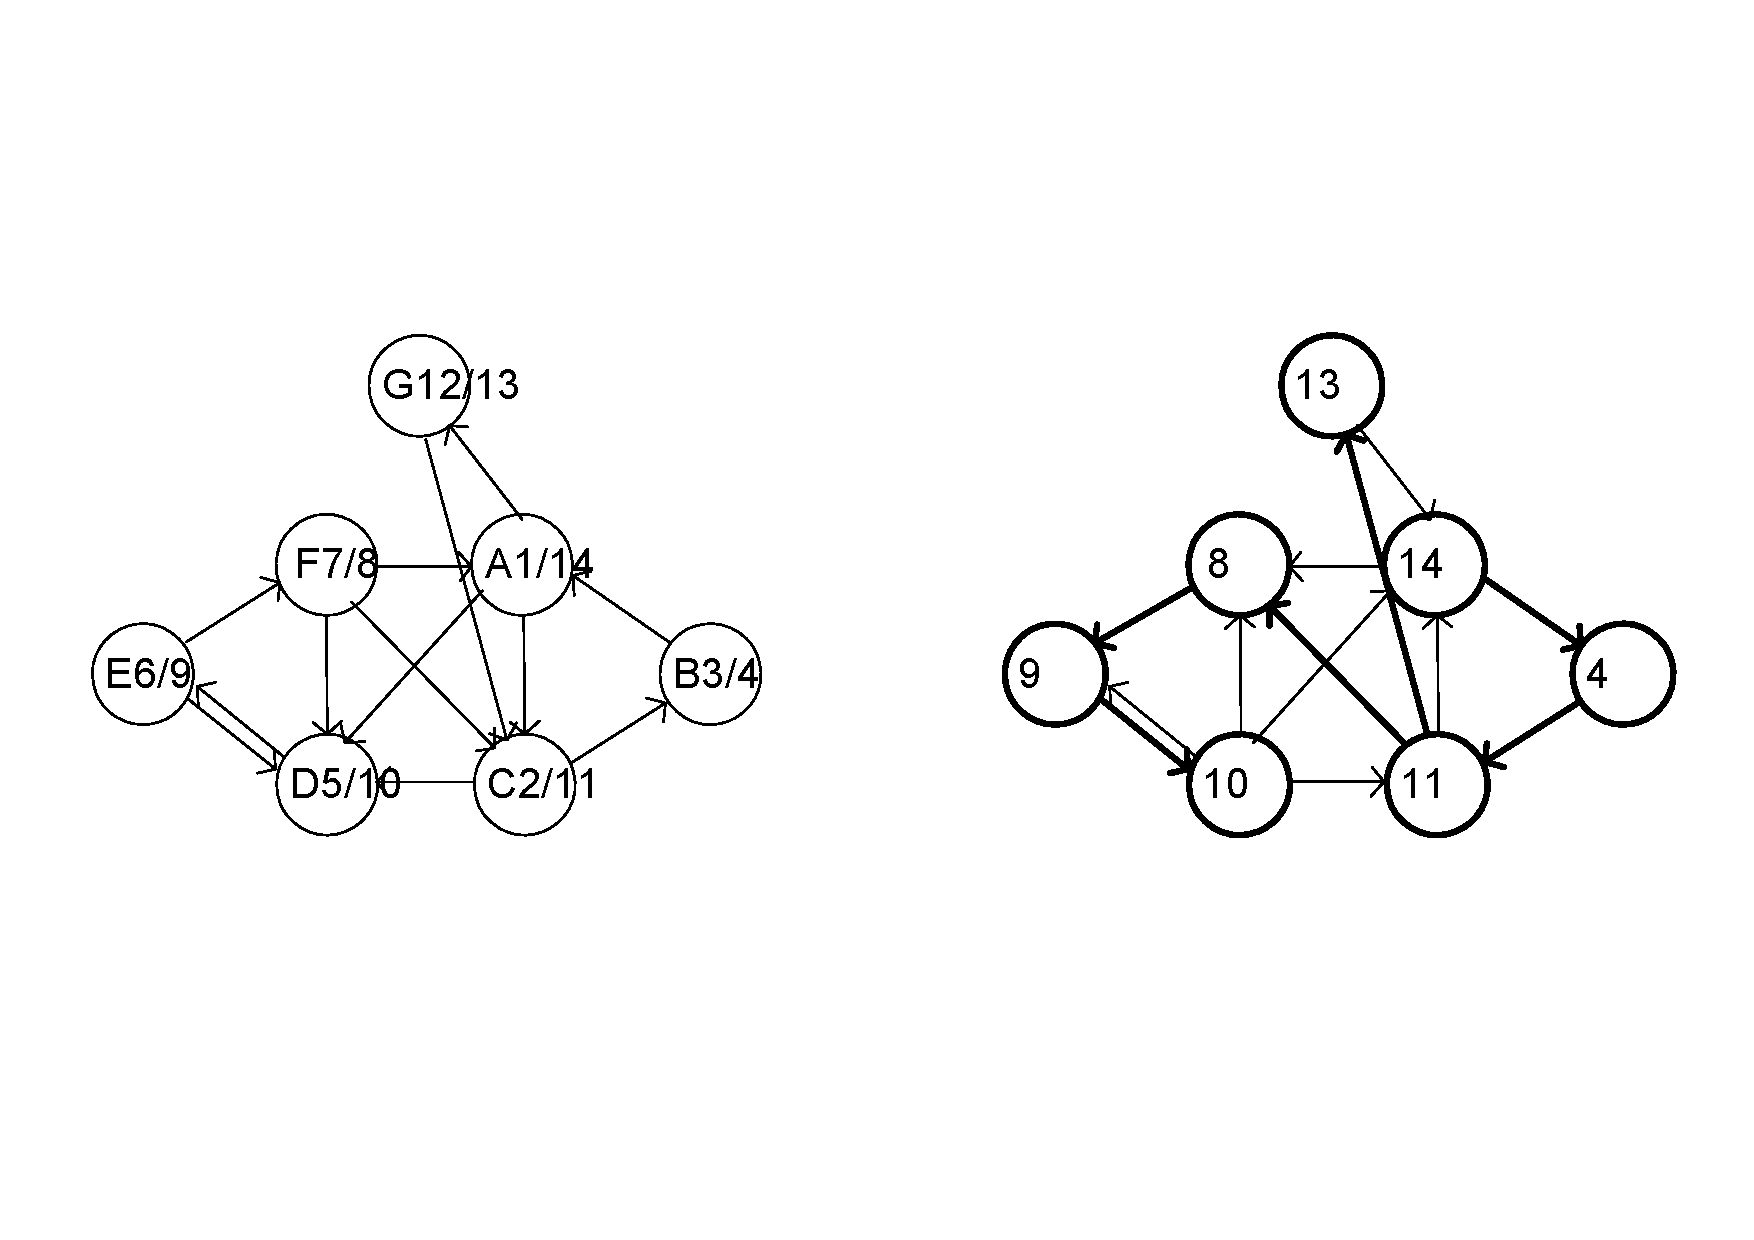
\includegraphics[width=\linewidth]{hw04Ex7}
	\caption{22.2-6}
	\label{fig:hw04Ex7}
\end{figure}

\section{Question 8: CLRS Problem Set 22.1}

\subsection{a-1}

Suppose $(v,u)$ is a backedge. u is ancestor elder than parent of v. This means $(s,u)$ + forwardEdge is shorter than $(s,v)$ produced by BFS which is $\delta(s,v)$ by \textbf{Theorem 22.5}. Same reason for forward edge.   

\subsection{a-2}

By \textbf{Theorem 22.5} $\delta(s,v) = \delta(s,v.parent) + (v.parent, v) = \delta(s,u) + (u,v) \rightarrow v.d = u.d + 1$

\subsection{a-3}

$v.d \le u.d + 1$ : Same as a-1, if $v.d > u.d + 1$, $\delta(s,v) = (s,u) + cross$ instead of $(s,v)$. \\
$v.d \ge u.d$: If $v.d < u.d$, $(v,u)$ should be find out first, since this is undirected graph. 

\subsection{b-1}

Same as a-1, the $(s, u) + backEdge$ would be shorter than $(s, v)$

\subsection{b-2}

Same as a-2, By \textbf{Theorem 22.5} $\delta(s,v) = \delta(s,v.parent) + (v.parent, v) = \delta(s,u) + (u,v) \rightarrow v.d = u.d + 1$

\subsection{b-3}

Only the first half of a-3. if $v.d > u.d + 1$, $\delta(s,v) = (s,u) + cross$ instead of $(s,v)$. 
\subsection{b-4}

By \textbf{Corollary 22.4} and By \textbf{Theorem 22.5}, we know that if v is an ancestor of u $\delta (s, u) = \delta(s, v) + k \rightarrow \delta(s, u) > \delta (s, v) \rightarrow u.d > v.d$, I did not see how $u.d = v.d$ but the statement is correct.

\section{Question 9: CLRS Problem Set 22.3}

\subsection{1. proof}

Euler tour exist $\rightarrow$ in-degree == out-degree: Suppose the cycle through i vertex n times would be $E-cycle = \{ v_{i}, v_{j}, v_{k}, ... , v_{i} \}$. The in-degree of $v_{j}$ would be the time of  $v_{j}$ appears with element in front, and out-degree of $v_{j}$ would be the time of $v_{j}$ appears with element in the back. If $v_{j}$ is not head or tail, this is obvious that every time $v_{j}$ appear, there is element in front and tail. If $v_{j}$ is head, it must also be tail, which balance the in-degree and out-degree again.\\

in-degree == out-degree $\rightarrow$ Euler tour exist

\subsection{2. implement}

This is very similar to SCC, we find closed cycle first then join them with other edge set. This procedure would return a cycle, which is a list of vertex. closed cycle has $cycle.begin() = cycle.end()$, open cycle(path, not a cycle) do not has it. But if Euler tour exist, open cycle would join close cycle into a big cycle.

\begin{codebox}
	
	\Procname{$\proc{CircleFind($cycle,u,v$)}$}
	\li $ClosedCycleSet, OpenCycleSet = \emptyset$
	\li \While $all adjList != \emptyset$ \Do
	\li \For $v$ in $Vertex$ with $adjList != \emptyset$\Do
	\li \If $v.adjList != \emptyset$ \Then
	\li new $cycle = \emptyset$
	\li \proc{CircleFindAid($cycle,u,NIL$)}
	\li \If $cycle.type == closed$
	\li \Then $ClosedCycleSet.push(cycle)$
	\li \Else $OpenCycleSet.push(cycle)$
	
\end{codebox}

\begin{codebox}
	
	\Procname{$\proc{CircleFindAid($cycle,u,v$)}$}
	\li $cycle.insert(u)$
	\li \If $v != NIL$ 
	\li \Then $v.adjList.erase(u)$ \End
	\li \If $u == NIL$ 
	\li \Then $cycle.type = open$
	\li \Return  
	\li \ElseIf $u == cycle.start$ 
	\li \Then $cycle.type = close$
	\li \Return 
	\li \Else $v = u$
	\li $u = u.adjList.begin()$
	\li \proc{CircleFind(cycle, u, v)}
	\End
	\End
	
\end{codebox}

It is easy to find that as we remove an edge from adjacent list once we find it, and we traverse every edge, the time complexity would be $\Theta(E)$

\section{Question 10: CLRS Exercise 12.2-1}
a. impossible since $\{330,344,397,363\}$ should be in left sub tree of node $338$\\
b. possible\\
c. impossible since$\{912, 245,363\}$ should be in left sub tree of node $911$\\
d. possible\\
e. impossible since $\{299, 392, 358, 363\}$ should be in right sub tree of node $347$

\section{Question 11: CLRS Exercise 12.2-5}
For successor: \textbf{if node X's right child has no left child}: then the successor would be X's right child which has no left child. \textbf{If node X's right child has left child}: then the successor would be the minimum element in the left sub tree of X's right child, which could not have left child or its left child would be less than it self.\\
For predecessor: same as successor.

\section{Question 12: CLRS Exercise 12.3-3}
Best case: $\Theta (nlogn)$ Consider a sorted sequence Each time we insert the median and slice into before median and after median, and do the same process recursively.\\ 
Worst cast: $\Theta(n^2)$ Consider constantly insert element at the end of a $List$. This could happen when we insert the $in-order$ traverse sequence either in an increase or decrease order. 

\section{Question 13: CLRS Exercise 12.3-3}

\subsection{a}
The value would be $\{16, 23, 7, 20\}$

\subsection{b}
For insertion, only one rotation would be triggered

\subsection{c}
See Figure~\ref{fig:hw04Ex13}

\begin{figure}
	\centering
	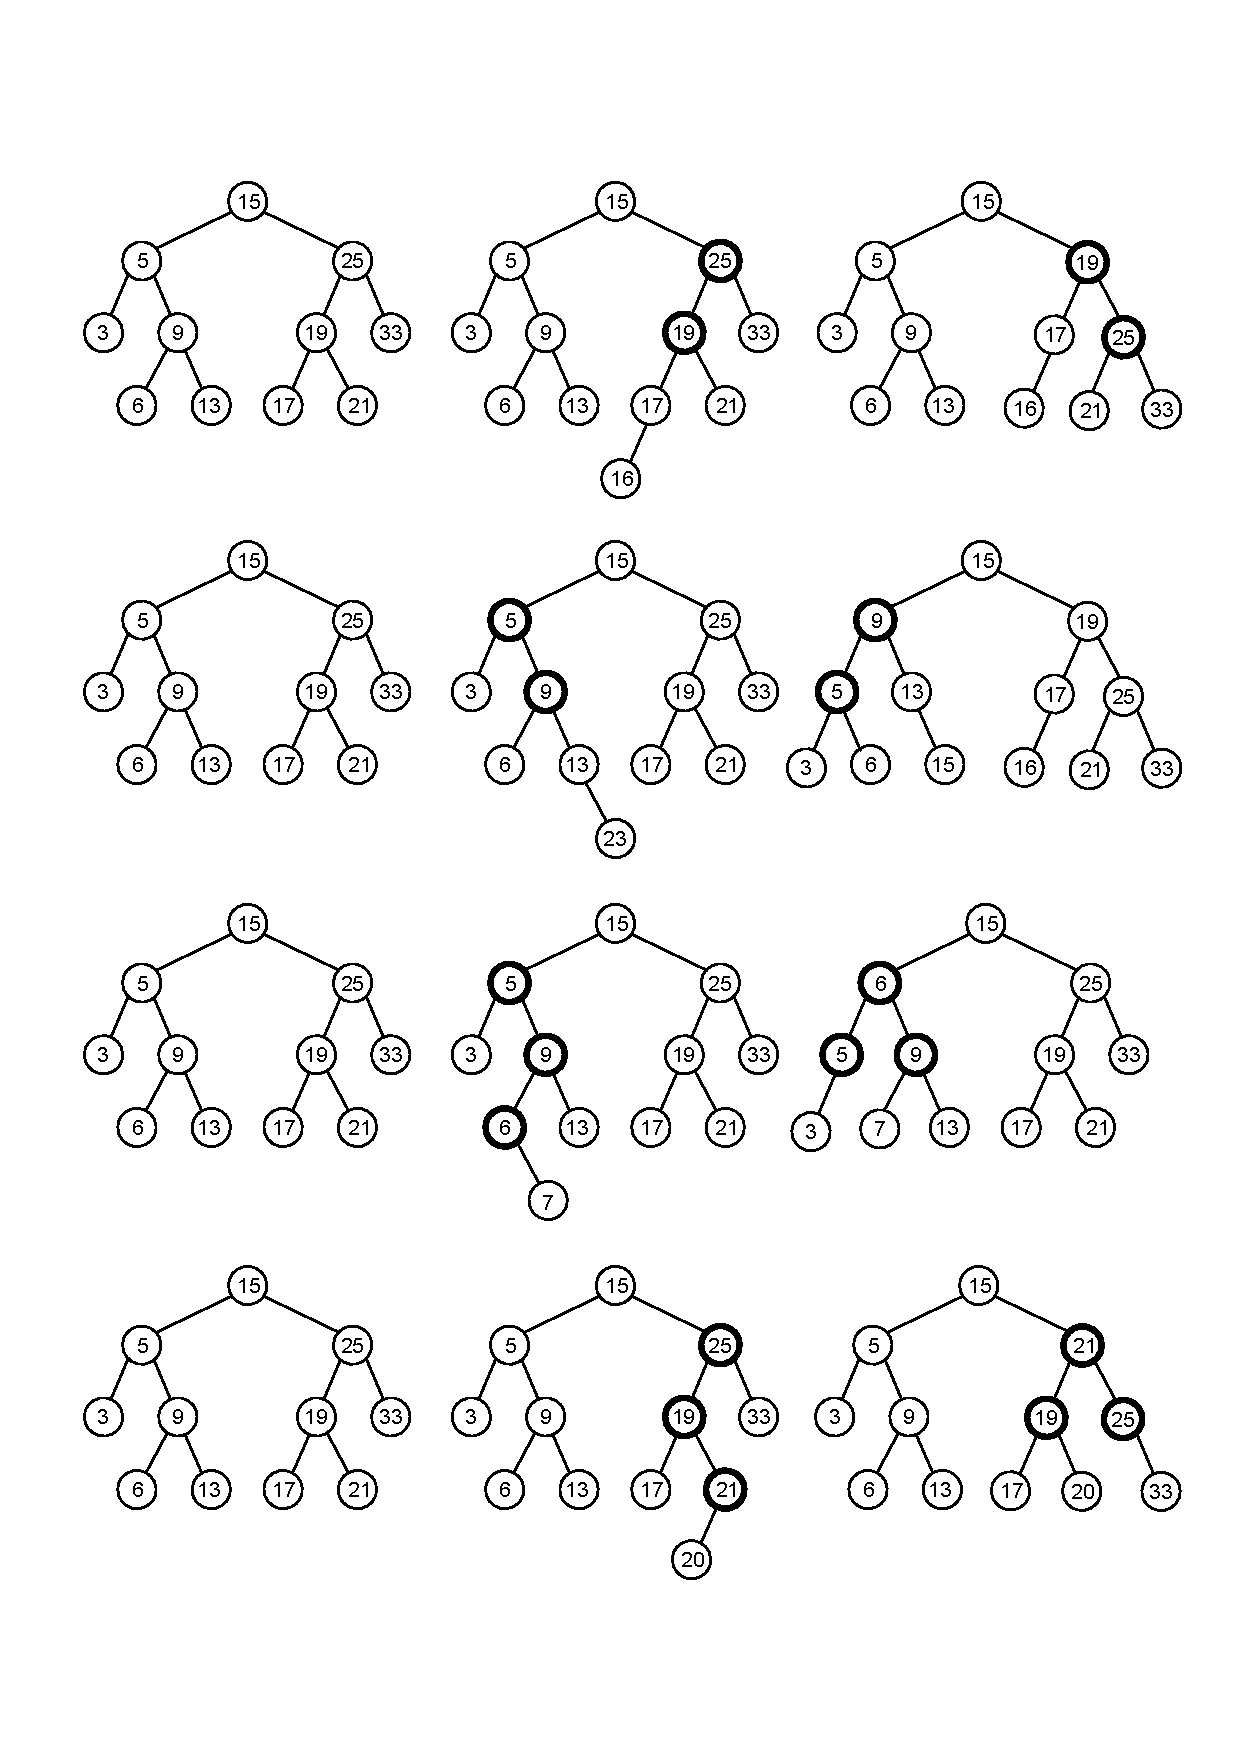
\includegraphics[width=\linewidth]{hw04Ex13}
	\caption{22.2-6}
	\label{fig:hw04Ex13}
\end{figure}


\end{document}
